\begin{abox}
	Assignment-S04\\
	\vspace{0.5cm}
	Multipole Expansion and Image Problem
	\end{abox}
\begin{enumerate}
	\item $\left. \right. $
	\begin{answer}
			(a) The monopole moment $Q=2 q-q=q$\\
		(b) The dipole moment of this configuration is $\vec{p}=2 q a \hat{y}$\\
		(c) The approximate potential (in spherical coordinates) at large distance $r$ is
		\begin{align*}
		V \approx \frac{1}{4 \pi \varepsilon_{0}}\left[\frac{Q}{r}+\frac{\vec{p} \cdot \hat{r}}{r^{2}}\right] \Rightarrow V \approx \frac{1}{4 \pi \varepsilon_{0}}\left[\frac{q}{r}+\frac{2 q a \sin \theta \sin \phi}{r^{2}}\right]
		\end{align*}
	\end{answer}
	\item $\left. \right. $
	 \begin{answer}
	 	\begin{align*}
	  \text{(a)}&\text{ The monopole moment }Q_{\text {mono }}=-\frac{q}{2}+q-\frac{q}{2}+q-q=0\\
	 	\text{(b) }&\text{The dipole moment}\text{ of this configuration is}\\
	 	\vec{p}&=q(a \hat{x}+a \hat{y})-\frac{q}{2}(-a \hat{x}+a \hat{y})+q(-a \hat{x}-a \hat{y})-\frac{q}{2}(a \hat{x}-a \hat{y})+0=0\\
	 	\text{(c) }&V \propto \frac{1}{r^{3}} \Rightarrow \frac{V(3 r)}{V(2 r)}=\frac{8}{27}
	 	\end{align*}
	 \end{answer}
	\item $\left. \right. $
	\begin{answer}
		 Let coordinates of $A$ is $(l, m)$, then
		\begin{align*}
		\vec{p}&=q_{i} \vec{r}_{i}^{\prime}=q[l \hat{i}+m \hat{j}]+2 q[(l+a) \hat{i}+m \hat{j}]-3 q\left[\left(l+\frac{a}{2}\right) \hat{i}+\left(m+\frac{\sqrt{3} a}{2}\right) \hat{j}\right] \\
		\vec{p}&=q[l \hat{i}+m \hat{j}]+2 q[(l+a) \hat{i}+m \hat{j}]-q\left[\left(3 l+\frac{3 a}{2}\right) \hat{i}+\left(3 m+\frac{3 \sqrt{3} a}{2}\right) \hat{j}\right] \\
		\Rightarrow \vec{p}&=\left(2 q a \hat{i}-\frac{3 q a}{2} \hat{i}\right)-\frac{3 \sqrt{3} q a}{2} \hat{j} \Rightarrow \vec{p}=\frac{q a}{2} \hat{i}-\frac{3 \sqrt{3} q a}{2} \hat{j}
		\end{align*}
	\end{answer}
	\item $\left. \right. $
	\begin{answer}
		\begin{align*}
		 \text{(a) }Q_{\text {mono }}&=\int_{S} \sigma d a=\int_{0}^{a} \int_{0}^{2 \pi}\left(\sigma_{0} r \cos \theta\right)(r d r d \theta)=0\\
		\text{(b) }p&=\int r^{\prime} \rho\left(r^{\prime}\right) d \tau^{\prime}=\int r^{\prime} \sigma\left(r^{\prime}\right) d a^{\prime}\\
		p_{x}&=\int x \sigma\left(r^{\prime}\right) d a^{\prime}=\iint(r \cos \theta) \times \sigma_{0} r \cos \theta d a^{\prime}=\int_{0}^{a} \int_{0}^{2 \pi} \sigma_{0} r^{2} \cos ^{2} \theta r d r d \theta \\
		p_{x}&=\sigma_{0} \int_{0}^{a} r^{3} d r \int_{0}^{2 \pi} \cos ^{2} \theta d \theta=\frac{\sigma_{0} a^{4}}{4} \times \pi=\frac{\sigma_{0} \pi a^{4}}{4}\\
		p_{y}&=\int y \sigma\left(r^{\prime}\right) d a^{\prime}=\iint(r \sin \theta) \times \sigma_{0} r \cos \theta d a^{\prime}=\int_{0}^{a} \int_{0}^{2 \pi} \sigma_{0} r^{2} \sin \theta \cos \theta r d r d \theta=0\\
		p_{x}&=\int z \sigma\left(r^{\prime}\right) d a^{\prime}=0\\
		\Rightarrow \vec{p}&=\frac{\sigma_{0} \pi a^{4}}{4} \hat{x}
		\end{align*}
	\end{answer}
	\item $\left. \right. $
	\begin{answer}
		\begin{align*}
		p&=\int_{V} r^{\prime} \rho\left(r^{\prime}\right) d \tau^{\prime}=\iiint r^{\prime} \times \rho_{0}\left(\frac{r_{0}}{r^{\prime}}\right)^{2} e^{-r^{\prime} / r_{0}} \cos ^{2} \varphi \times r^{\prime 2} \sin \theta d r^{\prime} d \theta d \varphi\\
		p&=\rho_{0} r_{0}^{2} \int_{r^{\prime}=0}^{\infty} r^{\prime} e^{-r^{\prime} / r_{0}} d r^{\prime} \int_{0}^{\pi} \sin \theta d \theta \int_{0}^{2 \pi} \cos ^{2} \varphi d \varphi=2 \pi \rho_{0} r_{0}^{4}
		\end{align*}
	\end{answer}
\item $\left. \right. $
	\begin{answer}
		(a) The magnitude of electric field at $(0,0, d)$ is $|\vec{E}|=\frac{2 q}{4 \pi \varepsilon_{0}(2 d)^{2}}=\frac{q}{8 \pi \varepsilon_{0} d^{2}}$\\
		(b) The work done in placing charge $2 q$ at $(0,0,-d)$ is
		\begin{align*}
		W&=\int_{\infty}^{d} \vec{F} \cdot d \vec{l}=\int_{\infty}^{d} \frac{2 q \times q}{8 \pi \varepsilon_{0} z^{2}} d z=-\frac{q^{2}}{4 \pi \varepsilon_{0} d}
			\end{align*}
			(c) There is attractive force between point charge $2 q$ and grounded conducting sheet that can be calculate from method of images i.e.
		\begin{align*}
		\frac{1}{4 \pi \varepsilon_{0}} \frac{(2 q)^{2}}{(2 d)^{2}}&=m g \Rightarrow d=\frac{q}{2 \sqrt{m g \pi \varepsilon_{0}}}
			\end{align*}
	\end{answer}
	\item $\left. \right. $
	\begin{answer}$\left. \right. $
		\begin{figure}[H]
			\centering
			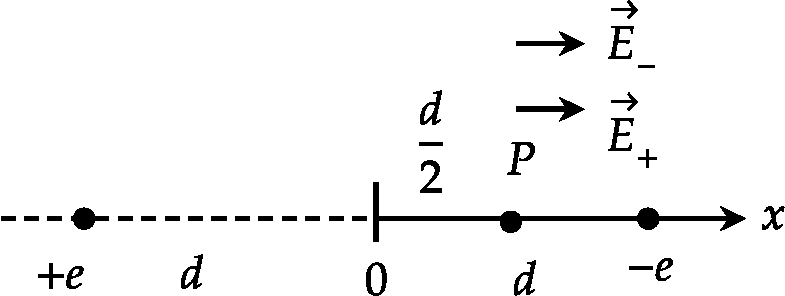
\includegraphics[height=2.4cm,width=6cm]{Assi-S15}
		\end{figure}
		\begin{align*}
		E_{+}&=\frac{1}{4 \pi \varepsilon_{0}} \frac{e}{(3 d / 2)^{2}}=\frac{1}{4 \pi \varepsilon_{0}} \frac{4 e}{9 d^{2}}\text{ and }E_{-}\\&=\frac{1}{4 \pi \varepsilon_{0}} \frac{e}{(d / 2)^{2}}=\frac{1}{4 \pi \varepsilon_{0}} \frac{4 e}{d^{2}}
		\intertext{Thus resultant electric field at point $P$ is}
		E&=E_{+}+E_{-}=\frac{1}{4 \pi \varepsilon_{0}} \frac{4 e}{9 d^{2}}+\frac{1}{4 \pi \varepsilon_{0}} \frac{4 e}{d^{2}}\\&=\frac{1}{4 \pi \varepsilon_{0}} \frac{40 e}{9 d^{2}}=\frac{1}{9 \pi \varepsilon_{0}} \frac{10 e}{d^{2}} \Rightarrow \vec{E}=\frac{1}{9 \pi \varepsilon_{0}} \frac{10 e}{d^{2}} \hat{x}
		\end{align*}
	\end{answer}
	\item $\left. \right. $
	\begin{answer}
			Using method of Images we can draw equivalent figure as shown below:
			\begin{figure}[H]
				\centering
				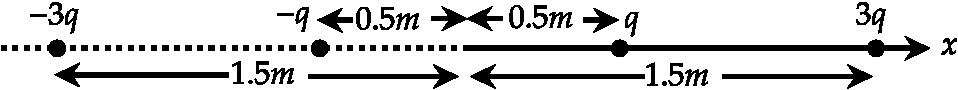
\includegraphics[height=1cm,width=10cm]{Assi-S16}
			\end{figure}
		\begin{align*}
	F&=\frac{q}{4 \pi \varepsilon_{0}}\left[\frac{3 q}{(1)^{2}}+\frac{q}{(1)^{2}}+\frac{3 q}{(2)^{2}}\right]=\frac{q}{4 \pi \varepsilon_{0}} \times \frac{19 q}{4}=\frac{1}{4 \pi \varepsilon_{0}} \frac{19 q^{2}}{4}
		\end{align*}
	\end{answer}
	\item $\left. \right. $
	\begin{answer}$\left. \right. $
			\begin{figure}[H]
			\centering
			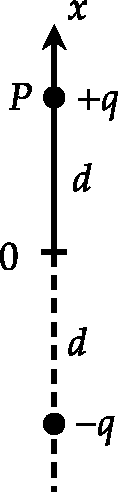
\includegraphics[height=4.7cm,width=1.2cm]{Assi-S17}
		\end{figure}
		\begin{align*}
	F&=m a=m \frac{d^{2} x}{d t^{2}}=-\frac{1}{4 \pi \varepsilon_{0}} \frac{q^{2}}{4 d^{2}} \Rightarrow \frac{d^{2} x}{d t^{2}}=-\frac{A}{x^{2}}\text{ where }A=\frac{q^{2}}{16 \pi m \varepsilon_{0}}.\\
		\Rightarrow \frac{d v}{d t}&=-\frac{A}{x^{2}} \Rightarrow v \frac{d v}{d t}=-\frac{A}{x^{2}} \frac{d x}{d t} \Rightarrow \frac{1}{2} \frac{d}{d t}\left(v^{2}\right)=\frac{d}{d t}\left(\frac{A}{x}\right) \\
		\Rightarrow \frac{v^{2}}{2}&=\frac{A}{x}+C \text { at } \Rightarrow x=d, v=0 \Rightarrow C=-\frac{A}{d} \Rightarrow v=\sqrt{2 A} \sqrt{\left(\frac{1}{x}-\frac{1}{d}\right)} . \\
		\text { Thus } u&=\sqrt{2 A} \sqrt{\left(\frac{1}{d / 4}-\frac{1}{d}\right)}=\sqrt{2 A} \sqrt{\frac{3}{d}} \Rightarrow \sqrt{2 A}=u \sqrt{\frac{d}{3}} \\
		\text { then } 2 u&=\sqrt{2 A} \sqrt{\left(\frac{1}{x}-\frac{1}{d}\right)} \Rightarrow 2 u=u \sqrt{\frac{d}{3}} \sqrt{\left(\frac{1}{x}-\frac{1}{d}\right)} \Rightarrow x=\frac{d}{13}\\
		\text{(b) }\because v&=\sqrt{2 A} \sqrt{\left(\frac{1}{x}-\frac{1}{d}\right)} \Rightarrow-\frac{d x}{d t}=\sqrt{2 A} \sqrt{\left(\frac{1}{x}-\frac{1}{d}\right)} \Rightarrow \int_{d}^{0} \sqrt{\frac{x d}{d-x}} d x=-\sqrt{2 A} \int_{0}^{t} d t\\
		\text{Put }x&=d \sin ^{2} \theta \Rightarrow d x=2 d \sin \theta \cos \theta d \theta\\
		\Rightarrow& \int_{\pi / 2}^{0} \sqrt{\frac{\left(d \sin ^{2} \theta\right) d}{d \cos ^{2} \theta}} 2 d \sin \theta \cos \theta d \theta=-\sqrt{2 A t} \\
		\Rightarrow-\sqrt{2 A} t&=\int_{\pi / 2}^{0} \sqrt{d} \frac{\sin \theta}{\cos \theta} 2 d \sin \theta \cos \theta d \theta=2 d^{3 / 2} \int_{\pi / 2}^{0} \sin ^{2} \theta d \theta \\
		\Rightarrow-\sqrt{2 A} t&=2 d^{3 / 2} \int_{\pi / 2}^{0} \frac{(1-\cos 2 \theta)}{2} d \theta=d^{3 / 2}\left[\theta-\frac{\sin 2 \theta}{2}\right]_{\pi / 2}^{0}=-d^{3 / 2} \frac{\pi}{2} \\
		\Rightarrow-\sqrt{2 A} t&=-d^{3 / 2} \frac{\pi}{2} \Rightarrow-\sqrt{\frac{q^{2}}{16 \pi m \varepsilon_{0}}} \times t=-d^{3 / 2} \frac{\pi}{2} \\
		\Rightarrow t&=d^{3 / 2} \frac{\pi}{2} \times \sqrt{\frac{8 \pi m \varepsilon_{0}}{q^{2}}}=\frac{\sqrt{2 \pi^{3} \varepsilon_{0} m d^{3}}}{q}
	\intertext{	Time taken by charge when it is released at a distance $d / 2$ is}
		t^{\prime}&=\frac{\sqrt{2 \pi^{3} \varepsilon_{0} m(d / 2)^{3}}}{q}=\frac{\sqrt{2 \pi^{3} \varepsilon_{0} m d^{3}}}{\sqrt{8} q}=\frac{t}{2 \sqrt{2}}
		\end{align*}
	\end{answer}
	\item $\left. \right. $
	\begin{answer}$\left. \right. $
		\begin{figure}[H]
			\centering
			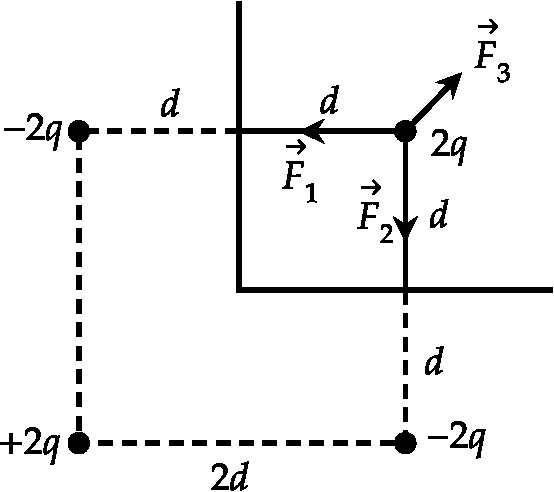
\includegraphics[height=4cm,width=4.5cm]{Assi-S18}
		\end{figure}
		\begin{align*}
		\left|\vec{F}_{1}\right|&=\left|\vec{F}_{2}\right|=k \frac{4 q^{2}}{4 d^{2}}=k \frac{q^{2}}{d^{2}}\text{ and }\left|\vec{F}_{3}\right|=k \frac{4 q^{2}}{8 d^{2}}=k \frac{q^{2}}{2 d^{2}}\\
		\text{ Resultant of }\vec{F}_{1}, \vec{F}_{2}\text{ is } F_{12}&=\sqrt{F_{1}^{2}+F_{2}^{2}}=\sqrt{2} k \frac{q^{2}}{d^{2}}.\\
		\text{Net force }\vec{F}&=k \frac{q^{2}}{d^{2}}\left(\sqrt{2}-\frac{1}{2}\right)=\frac{q^{2}}{8 \pi \varepsilon_{0} d^{2}}(2 \sqrt{2}-1)\\
		\text{ (towards the corner)}&
		\end{align*}
	\end{answer}
	
	
	
	
	
	
	
	
	
	
	
	
\end{enumerate}